\documentclass[conference]{IEEEtran}
\IEEEoverridecommandlockouts
% The preceding line is only needed to identify funding in the first footnote. If that is unneeded, please comment it out.
\usepackage{cite}
\usepackage{amsmath,amssymb,amsfonts}
\usepackage{algorithmic}
\usepackage{graphicx}
\usepackage{textcomp}
\usepackage{xcolor}
\usepackage{booktabs}  % for \toprule, \midrule, \bottomrule
\usepackage{caption}   % nicer caption formatting
\usepackage{url}       % For URL formatting in bibliography
\def\BibTeX{{\rm B\kern-.05em{\sc i\kern-.025em b}\kern-.08em
    T\kern-.1667em\lower.7ex\hbox{E}\kern-.125emX}}
\begin{document}

\title{Developing and Evaluating Rule-Based and Reinforcement Learning Agents for the Game of Hex}

\author{\IEEEauthorblockN{Salome Christiani}
\IEEEauthorblockA{\textit{FH Technikum Wien} \\
\textit{Master AI \& Game Engineering}\\
Wien, AT \\
ai24m057@technikum-wien.at}
\and
\IEEEauthorblockN{Nikolaus Rieder}
\IEEEauthorblockA{\textit{FH Technikum Wien} \\
\textit{Master AI \& Game Engineering}\\
Wien, AT \\
ai24m040@technikum-wien.at}
}

\maketitle

\begin{abstract}
This paper presents the development and evaluation of agents for playing the Hex board game. We explore two distinct approaches: first, crafting strong, interpretable rule-based heuristic agents that serve as robust baselines, and second, training a learning-based agent using Proximal Policy Optimization (PPO). The rule-based agents employ a sophisticated weighted voting system over a set of tactical and strategic heuristics, such as bridge detection, pathfinding, and threat analysis. These agents were then utilized as opponents in a curriculum learning setup for the PPO agent. The main objective was to train a PPO agent capable of outperforming these heuristic baselines, with the ultimate goal of competing in a class-wide 7x7 Hex tournament. Our findings indicate that while the PPO agent successfully learned to defeat random and our bespoke rule-based opponents, it struggled with defensive awareness and long-term strategic planning, often failing to recognize and block opponent threats. This work highlights the challenges of learning complex game strategies from sparse rewards and lays the foundation for future improvements through hybrid learning approaches. The project also features a modular, interactive visualization framework to support development, debugging, and evaluation across various play modes.
\end{abstract}

\begin{IEEEkeywords}
Hex, Reinforcement Learning, Proximal Policy Optimization (PPO), Rule-Based Systems, Game AI, Heuristics
\end{IEEEkeywords}

\section{Introduction}
Hex is a two-player, zero-sum, perfect information connection game with a surprisingly high strategic depth despite its simple rules \cite{b1}. This makes it an ideal testbed for exploring artificial intelligence techniques. The game's large state space and the subtle nature of its strategies present a compelling challenge for both classical AI and modern machine learning approaches.

This project undertakes a comparative study of two primary paradigms for creating Hex-playing agents. The first is a classical, knowledge-based approach, resulting in the development of sophisticated \textbf{rule-based agents}. These agents are designed to mimic human-like heuristics and tactical reasoning, providing a strong, interpretable baseline for performance. The second approach leverages state-of-the-art \textbf{Reinforcement Learning (RL)}, specifically Proximal Policy Optimization (PPO), to train an agent from experience. The motivation for this dual approach is to understand the trade-offs between engineered knowledge and learned policies. While rule-based systems are transparent and can be finely tuned, they are limited by the explicit knowledge encoded by their creators. In contrast, RL agents have the potential to discover novel, superhuman strategies but often act as "black boxes" and can struggle to learn fundamental concepts like defense without careful reward shaping and extensive training.

Our primary goal was to develop a PPO agent that could not only learn the game but also surpass the performance of our own handcrafted rule-based systems. These rule-based agents served a dual purpose: as a benchmark for performance and as structured, challenging opponents during the RL training process, creating a curriculum to guide the learning agent. This paper details the architecture of both agent types, the experimental setup for training the PPO agent, and a thorough analysis of the results, culminating in a discussion of the observed strengths and weaknesses of each approach.

\section{Methods}
This section details the technical implementation of the core components of our project: the game environment, the rule-based agents, and the reinforcement learning agent.

\subsection{Game Engine and Visualization}
At the core of the project is a custom game engine, encapsulated in the \texttt{hexPosition} class. This class manages the board state, enforces game rules, detects win conditions, and maintains a history of moves. The engine is designed to be modular and supports a 7x7 board size for the competition.

To facilitate development, debugging, and analysis, we integrated a visualization framework using Pygame. This GUI provides an interactive board where one can:
\begin{itemize}
    \item Play against any of the developed agents (human-vs-machine).
    \item Observe matches between two agents (machine-vs-machine).
    \item Step through games move by move or let them play out automatically.
    \item Export videos of gameplay for later review.
\end{itemize}
This interactive tool proved invaluable for qualitatively assessing agent behavior and identifying strategic flaws.

% TODO: [Insert a figure showing the Pygame GUI in action, perhaps a screenshot of a mid-game state.]
\begin{figure}[htbp]
\centerline{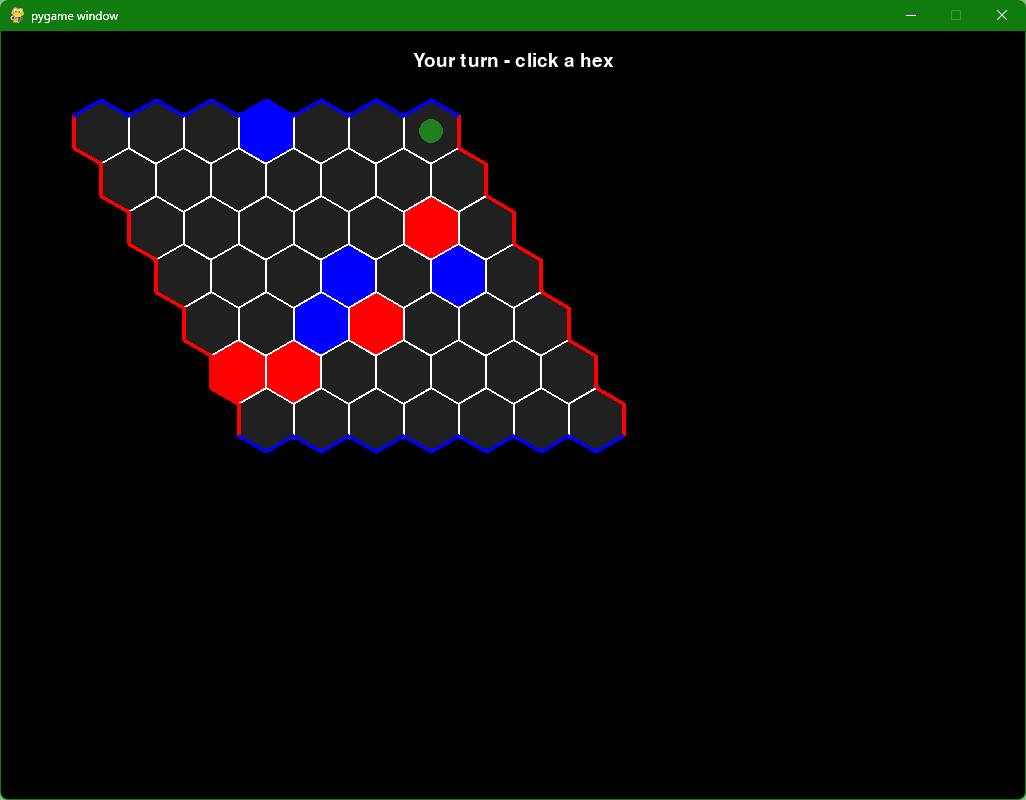
\includegraphics[width=0.8\columnwidth]{hex-pygame.png}}
\caption{The Pygame visualization framework showing a game in progress.}
\label{fig:gui}
\end{figure}

\subsection{Rule-Based Heuristic Agents}
We developed two primary versions of a rule-based agent, \texttt{v3} and \texttt{v4}, to serve as strong baselines and as training opponents for the RL agent. These agents are not based on simple, hardcoded rules but on a dynamic, weighted evaluation of multiple strategic heuristics.

\subsubsection{Strategy Framework}
The core of the rule-based agents is a collection of functions, each representing a specific tactical or strategic concept in Hex. At each turn, every strategy function is called to suggest a move. The main strategies include:
\begin{itemize}
    \item \textbf{Immediate Win/Block Detection:} Checks for moves that result in an immediate win or are necessary to block an opponent's immediate win. These are given the highest priority.
    \item \textbf{Forcing Moves:} Identifies moves that guarantee a win within the next two turns.
    \item \textbf{Pathfinding and Connectivity:}
          \begin{itemize}
              \item \textit{Shortest Connection Path:} Uses a Numba-accelerated Dijkstra's algorithm to find the shortest potential path to the goal and suggests moves along it.
              \item \textit{Extend Own Chain:} Identifies the agent's most promising chain and extends it.
              \item \textit{Protect Own Chain from Cut:} Reinforces weak points in the agent's own connection.
          \end{itemize}
    \item \textbf{Bridge Tactics:}
          \begin{itemize}
              \item \textit{Make Own Bridge:} Proactively creates bridge patterns to form robust connections \cite{b5}.
              \item \textit{Break Opponent Bridge:} Identifies and blocks the opponent's bridge formations.
          \end{itemize}
    \item \textbf{Positional and Threat-Based Heuristics:}
          \begin{itemize}
              \item \textit{Create Double Threat:} Finds moves that create two simultaneous threats.
              \item \textit{Take Center:} Prioritizes central board control in the opening phase.
              \item \textit{Block Aligned Opponent Path:} Disrupts the opponent's main axis of attack.
          \end{itemize}
\end{itemize}

\subsubsection{Weighted Voting and Game Phase Adaptation}
Instead of a rigid hierarchy, the agent uses a weighted voting system. Each strategy's suggestion contributes to a score for its proposed move. The final move is chosen from the highest-scoring candidates.

Crucially, the weights assigned to each strategy are not static. They adapt based on the current \textbf{game phase}, which is determined by the number of stones on the board (Opening, Mid-Game, End-Game). For example, \texttt{take\_center} is heavily weighted in the first few moves, while \texttt{create\_double\_threat} becomes more important in the late game. The key difference between agent versions \texttt{v3} and \texttt{v4} lies in the fine-tuning of these weights, with \texttt{v4} placing a greater emphasis on late-game disruption and blocking.

\subsection{Reinforcement Learning Agent}
The primary learning-based agent was developed using the Proximal Policy Optimization (PPO) algorithm, a state-of-the-art RL method known for its stability and sample efficiency.

\subsubsection{Model Architecture and Observation Space}
The agent's brain is a neural network that takes the state of the board as input and outputs a policy (a probability distribution over possible moves).
\begin{itemize}
    \item \textbf{Observation Space:} The board is represented as a 3-channel tensor of shape (3, 7, 7). The channels represent the locations of Player 1's stones, Player -1's stones, and a plane indicating whose turn it is. This multi-channel representation allows the network to distinguish between players and the current game context.
    \item \textbf{Feature Extractor (\texttt{HexCNN}):} We designed a custom Convolutional Neural Network (CNN), \texttt{HexCNN}, to process this input. It consists of two \texttt{Conv2d} layers with ReLU activations. CNNs are well-suited for board games as they can learn spatial patterns and relationships between pieces, which is essential for understanding the game's topology.
    \item \textbf{Policy and Value Heads:} The features extracted by the CNN are fed into two separate fully connected (MLP) heads: a policy head that determines the next move, and a value head that estimates the probability of winning from the current state.
\end{itemize}

% TODO: [Insert a figure illustrating the PPO agent's model architecture: Input Tensor -> HexCNN -> MLP -> Policy/Value Heads.]
% \begin{figure}[htbp]
% \centerline{\includegraphics[width=\columnwidth]{model_architecture.png}}
% \caption{The neural network architecture for the PPO agent.}
% \label{fig:arch}
% \end{figure}

\subsubsection{Training Environment and Process}
The agent was trained using the \texttt{stable-baselines3} \cite{b2} and \texttt{sb3-contrib} libraries, within a \texttt{Gymnasium} \cite{b3} environment.
\begin{itemize}
    \item \textbf{Action Masking:} A key challenge in Hex is that the number of legal moves decreases as the game progresses. To handle this, we used \texttt{MaskablePPO}, a variant of PPO that accepts an "action mask" at each step. This ensures the agent only considers valid moves, preventing wasted exploration and making learning more efficient.
    \item \textbf{Vectorized Environments:} To accelerate training, we ran up to 16 game environments in parallel using \texttt{SubprocVecEnv}.
    \item \textbf{Opponent Curriculum:} The agent was trained against a mix of opponents, including the random agent and our rule-based \texttt{v3} and \texttt{v4} agents. This curriculum exposes the agent to a range of playstyles, from chaotic to structured, fostering more robust and generalizable strategies.
    \item \textbf{Unified Two-Player Wrapper:} To mitigate the significant first-player advantage and ensure the agent learns from both perspectives, we implemented a custom \texttt{SideSwapWrapper}. This wrapper encapsulates a full round of play (agent move + opponent response) and handles the random assignment of the agent to Player 1 or Player 2 at the start of each episode. When the agent is Player 2, the wrapper automatically flips observations, actions, and rewards to a canonical Player 1 perspective, allowing the agent to learn a single, unified policy.
\end{itemize}

\section{Evaluation}
To assess the performance of our agents and the effectiveness of our training methodologies, we conducted a series of structured experiments. The primary goal was to measure the learning progression of the PPO agent against various benchmarks. For all experiments, the board size was fixed at 7x7, and training was conducted using the PPO algorithm with the \texttt{MaskablePPO} implementation. The evaluation metric for all experiments is the mean reward against a static, strong opponent: our \texttt{rule\_based\_v4\_agent}.

\subsection{Experiment 1: Fixed-Side vs. Random Opponent}
\begin{itemize}
    \item \textbf{Objective:} To establish a baseline for learning by training the agent from a single perspective against a purely random opponent.
    \item \textbf{Methodology:} The \texttt{OpponentWrapper} was used, fixing the agent to always play as Player 1. The opponent pool consisted of 100\% random agents. The agent was trained for 500 thousand timesteps.
\end{itemize}

\subsection{Experiment 2: Side-Swapped vs. Random Opponent}
\begin{itemize}
    \item \textbf{Objective:} To measure the impact of perspective generalization by forcing the agent to learn strategies for both sides of the board.
    \item \textbf{Methodology:} The \texttt{SideSwapWrapper} was used to randomly assign the agent to be Player 1 or Player 2 in each episode. The opponent pool remained 100\% random. The agent was trained for 500 thousand timesteps.
\end{itemize}

\subsection{Experiment 3 & 4: Curriculum Learning with Rule-Based Opponents}
\begin{itemize}
    \item \textbf{Objective:} To test the hypothesis that training against a curriculum of increasingly strategic opponents improves final performance.
    \item \textbf{Methodology:} Two experiments were run using the \texttt{SideSwapWrapper}.
        \begin{itemize}
            \item \textbf{E3:} The opponent pool was 50\% rule-based agents (v3/v4) and 50\% random.
            \item \textbf{E4:} The opponent pool was 90\% rule-based agents and 10\% random.
        \end{itemize}
    Both agents were trained for 500 thousand timesteps to allow for convergence against the more difficult opponents.
\end{itemize}

\subsection{Experiment 5: Self-Play against Best Predecessor}
\begin{itemize}
    \item \textbf{Objective:} To simulate an "arms race" where the agent is forced to improve upon its own strongest previously learned policy.
    \item \textbf{Methodology:} The best-performing model from Experiment 4 was used as the sole opponent for a new training run. The \texttt{SideSwapWrapper} was used, and the agent was trained for 500 thousand timesteps. This setup tests if the agent can find and exploit weaknesses in its own past strategies.
\end{itemize}

\section{Results}
This section presents the outcomes of our experiments, focusing on the performance of the PPO agent and the insights gained from its behavior, as observed through our TensorBoard logs.

\subsection{Overall Performance Against the Rule-Based v4 Agent}
The primary metric for success, \texttt{eval/mean\_reward}, clearly demonstrates the effectiveness of our curriculum learning approach.
\begin{itemize}
    \item \textbf{E1 (Fixed-Side vs. Random):} This agent performed poorly in evaluation, achieving a final mean reward of approximately -0.9. This confirms that learning against only random opponents from a single perspective does not prepare the agent for strategic play.
    \item \textbf{E2 (Side-Swapped vs. Random):} Introducing side-swapping improved generalization slightly, but the agent still struggled against the v4 opponent, with a final mean reward of roughly -0.7.
    \item \textbf{E3 (50\% Rules Curriculum):} The introduction of rule-based opponents had a significant positive impact. The agent's performance steadily climbed, reaching a stable mean reward of approximately +0.2, indicating it was winning more often than losing against the strong baseline.
    \item \textbf{E4 (90\% Rules Curriculum):} Increasing the proportion of rule-based opponents further boosted performance. This agent achieved the highest evaluation score, with a final mean reward plateauing around +0.6. This strongly suggests that training against a challenging and structured curriculum is the most effective method.
    \item \textbf{E5 (Self-Play):} The self-play agent's performance was comparable to the E3 agent, with a final evaluation reward around +0.15. While it did not surpass the E4 agent, its training \texttt{rollout/ep\_rew\_mean} hovered consistently around 0.0, indicating a healthy and stable self-play dynamic where it was evenly matched against its predecessor.
\end{itemize}
% TODO: [Insert a figure comparing the \texttt{eval/mean_reward} curves for all 5 experiments.]
\begin{figure}[htbp]
\centerline{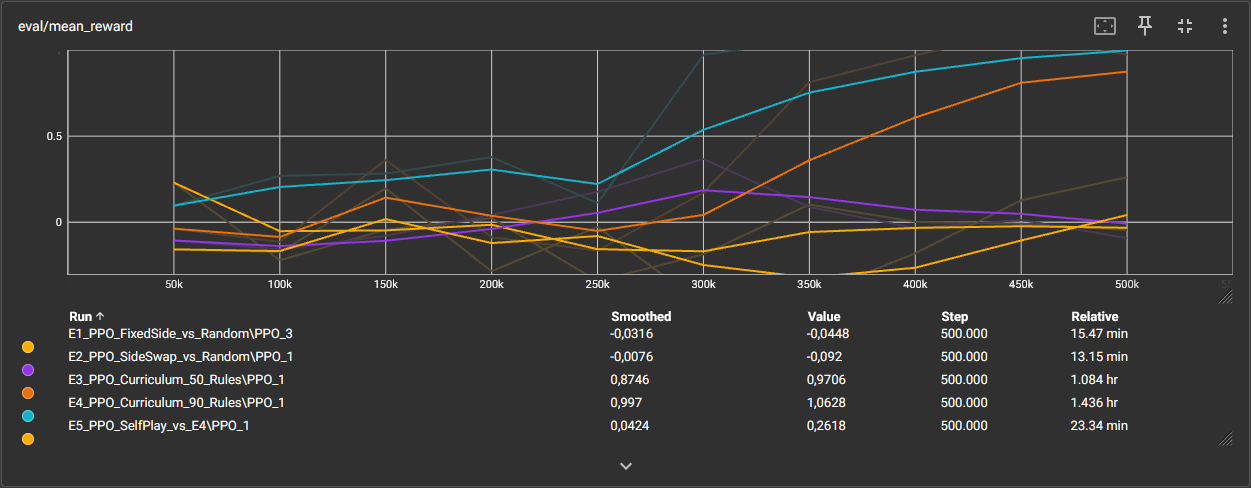
\includegraphics[width=\columnwidth]{eval-mean-reward_allRuns.png}}
\caption{Comparison of \texttt{eval/mean\_reward} across all experiments. The evaluation opponent is always the \texttt{rule\_based\_v4\_agent}.}
\label{fig:eval_reward}
\end{figure}

\subsection{Analysis of Learned Strategies}
By logging when the PPO agent's chosen move matched a heuristic suggestion, we can infer which strategies it learned independently.
\begin{itemize}
    \item \textbf{Basic Heuristics:} Across all curriculum experiments (E3, E4, E5), the agent quickly learned to replicate simple, high-value heuristics. The \texttt{agent\_matches\_extend\_own\_chain} and \texttt{agent\_matches\_shortest\_connection} metrics showed a clear upward trend, indicating the agent learned the fundamental concept of creating and advancing a connection.
    \item \textbf{Advanced Heuristics:} The agent also showed evidence of learning more complex tactics. The \texttt{agent\_matches\_break\_opponent\_bridge} metric increased steadily, especially in the E4 run, showing the agent learned the importance of this key defensive maneuver.
    \item \textbf{Limitations:} However, metrics for highly abstract or multi-turn strategies, such as \texttt{agent\_matches\_create\_double\_threat}, remained low across all experiments. This suggests that while the agent learned to react to local patterns, it struggled to develop deep, long-term plans.
\end{itemize}
% TODO: [Insert a figure showing the curves for \texttt{agent_matches_shortest_connection} and \texttt{agent_matches_break_opponent_bridge} for the E4 run.]
% \begin{figure}[htbp]
% \centerline{\includegraphics[width=\columnwidth]{strategy_matches.png}}
% \caption{Evolution of the PPO agent's alignment with key heuristics during the E4 training run.}
% \label{fig:strategy_match}
% \end{figure}

\subsection{Observed Strategic Weaknesses}
Despite its successes, qualitative analysis of the PPO agent's gameplay revealed two significant and persistent weaknesses:
\begin{enumerate}
    \item \textbf{Lack of Defensive Urgency:} The agent frequently failed to identify and block direct, winning threats from the opponent. Unless a defensive move also aligned with its own offensive goals (e.g., it also happened to be on its shortest path), it would often ignore the threat, leading to a loss. This suggests the sparse win/loss reward was insufficient to teach the agent the value of proactive defense.
    \item \textbf{No Multi-Turn Strategic Planning:} The PPO agent played reactively, optimizing its policy for the current board state. It struggled to maintain a coherent, multi-turn strategy. For instance, it might start building a promising bridge but abandon it on the next turn for a move that seemed locally optimal but was strategically inferior. This contrasts sharply with the rule-based agents, which could follow through on plans like the \texttt{shortest\_connection} path.
\end{enumerate}
Manual test games against the final PPO agent confirmed these observations. It was often possible to defeat the agent by setting up a simple threat that it would fail to block.

\section{Discussion}
This project successfully developed and evaluated two distinct types of AI agents for the game of Hex. Our work provides a clear comparison between a knowledge-driven, heuristic approach and a data-driven, reinforcement learning approach.

The rule-based agents, particularly \texttt{v4}, proved to be formidable opponents. Their strength lies in their explicit encoding of human-understandable strategies and their ability to follow a consistent plan. The dynamic, phase-aware weighting system allowed them to adapt their priorities effectively throughout the game, making them robust and difficult to exploit.

The PPO agent, on the other hand, demonstrated the power of reinforcement learning to master a complex game from scratch. Its ability to defeat the rule-based agents, especially in the E4 experiment, is a testament to the effectiveness of the PPO algorithm and our training setup. The use of a challenging opponent curriculum, action masking, and the custom \texttt{HexCNN} architecture were all critical to this success.

However, the results also highlight the limitations of a pure RL approach in a game that requires deep strategic foresight and a balance between offense and defense. The agent's primary weaknesses—poor defensive awareness and a lack of long-term planning—are indicative of the challenges of learning from a sparse reward signal. The agent learned *what* moves are associated with winning states but not always *why* they are good, leading to brittle and exploitable strategies.

In conclusion, while our PPO agent showed great promise and an ability to learn complex heuristics, the handcrafted rule-based agent remained a more reliable and strategically coherent player in certain situations. This suggests that the most promising path forward may lie in combining the strengths of both paradigms.

\subsection{Future Work}
Based on our findings, several avenues for future research could address the observed weaknesses:
\begin{itemize}
    \item \textbf{Hybrid Models:} A hybrid agent could use the rule-based system to generate candidate moves or provide a strategic prior, which the RL policy could then refine. For example, the RL agent could learn to choose between the top suggestions from the heuristic strategies.
    \item \textbf{Advanced Search Techniques:} Integrating the learned policy with a search algorithm like Monte Carlo Tree Search (MCTS), as famously done in AlphaGo, could provide the long-term planning capabilities that the current agent lacks.
    \item \textbf{Improved Reward Shaping:} Designing more sophisticated reward functions that explicitly reward defensive maneuvers or penalize the failure to block threats could help the agent learn a more balanced style of play.
    \item \textbf{More Extensive Curriculum Learning:} A more granular curriculum, with a wider variety of specialized opponents (e.g., purely aggressive, purely defensive), could help the agent learn a more complete set of skills.
\end{itemize}
The framework and agents developed in this project \cite{b4} provide a solid foundation for exploring these and other advanced topics in the fascinating domain of game AI.

\section*{Acknowledgment}
We would like to express our sincere gratitude to our instructor, \textbf{De Oliveira Gomes Rosana}, for their valuable guidance, insightful feedback, and continuous support throughout this project. Their expertise and encouragement played a crucial role in shaping both our technical approach and understanding of reinforcement learning in strategic games.

\begin{thebibliography}{00}
\bibitem{b1} Wikipedia, ``Hex (board game),'' Wikimedia Foundation. [Online]. Available: \url{https://en.wikipedia.org/wiki/Hex_(board_game)}
\bibitem{b2} A. Raffin, A. Hill, A. Gleave, A. Kanervisto, M. Ernestus, and N. Dormann, ``Stable-Baselines3: Reliable Reinforcement Learning Implementations,'' \textit{Journal of Machine Learning Research}, vol. 22, no. 268, pp. 1-8, 2021.
\bibitem{b3} J. Terry, et al., ``Gymnasium,'' Farama Foundation, 2023. [Online]. Available: \url{https://gymnasium.farama.org/}
\bibitem{b4} S. Christiani and N. Rieder, ``REIL-hex-game,'' GitHub Repository, 2024. [Online]. Available: \url{https://github.com/HackXIt/REIL-hex-game}
\bibitem{b5} BiffsGamingVideos, ``How to Play Hex - And Basic Strategy,'' YouTube, Oct. 2, 2017. [Online]. Available: \url{https://www.youtube.com/watch?v=8JNP8T7kCW}
\end{thebibliography}

\end{document}
